\documentclass[12pt]{extarticle}
\usepackage{physics}
\usepackage{yquant}

\title{Example Document}
\author{Some One}
\date{January 2025}

\begin{document}
\maketitle
\section{Example}
\begin{figure}[h]
    \centering
    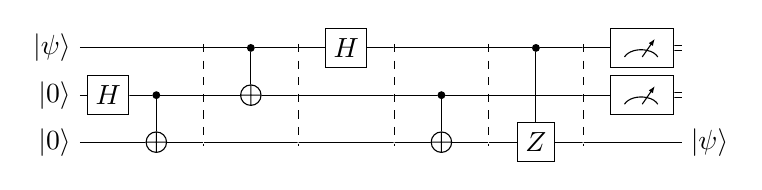
\begin{tikzpicture}
        \begin{yquant}
            qubit {$\ket{\psi}$} q0;
            qubit {$\ket{0}$} q1;
            qubit {$\ket{0}$} q2;
            h q1;
            cnot q2 | q1;
            barrier (-);
            cnot q1 | q0;
            barrier (-);
            h q0;
            barrier (-);
            cnot q2 | q1;
            barrier (-);
            z q2 | q0;
            barrier (-);
            measure q0;
            measure q1;
            output {$\ket{\psi}$} q2;
        \end{yquant}
        \end{tikzpicture}
    \caption{Teleportation}
    \label{fig:teleportation}
\end{figure}
\end{document}
